\documentclass{beamer}
\usepackage[backend=bibtex,style=numeric,sorting=none]{biblatex}
\usepackage{progressbar}
\usepackage[final]{listings}
\usepackage{graphicx}
\usepackage{hyperref}
\usepackage{pdfpages}
\graphicspath{ {./images/} }

\addbibresource{main.bib}
\usetheme{AnnArbor}

\title{Docker}
\subtitle{Information security club course \RN{2}}
\author{Chih-Hsuan Yang(SCC)}
\institute{National Sun Yat-sen University}
\date{\today\\v0.1}

\AtBeginSection[]{
    \begin{frame}
        \vfill
        \centering
        \begin{beamercolorbox}[sep=8pt,center,shadow=true,rounded=true]{title}
          \usebeamerfont{title}\insertsectionhead\par
        \end{beamercolorbox}
        \vfill
        \end{frame}
}

\definecolor{mygreen}{rgb}{0,0.6,0}
\definecolor{mygray}{rgb}{0.5,0.5,0.5}
\definecolor{mymauve}{rgb}{0.58,0,0.82}

% Code conf.
\lstset{ 
  backgroundcolor=\color{white},   % choose the background color; you must add \usepackage{color} or \usepackage{xcolor}; should come as last argument
  basicstyle=\ttfamily\footnotesize,% the size of the fonts that are used for the code
  breakatwhitespace=false,         % sets if automatic breaks should only happen at whitespace
  breaklines=true,                 % sets automatic line breaking
  captionpos=b,                    % sets the caption-position to bottom
  commentstyle=\color{mygreen},    % comment style
  deletekeywords={...},            % if you want to delete keywords from the given language
  escapeinside={\%*}{*)},          % if you want to add LaTeX within your code
  extendedchars=true,              % lets you use non-ASCII characters; for 8-bits encodings only, does not work with UTF-8
  frame=single,	                   % adds a frame around the code
  keepspaces=true,                 % keeps spaces in text, useful for keeping indentation of code (possibly needs columns=flexible)
  keywordstyle=\color{red},       % keyword style
  morekeywords={*,...},            % if you want to add more keywords to the set
  numbers=left,                    % where to put the line-numbers; possible values are (none, left, right)
  numbersep=5pt,                   % how far the line-numbers are from the code
  numberstyle=\tiny\color{mygray}, % the style that is used for the line-numbers
  rulecolor=\color{black},         % if not set, the frame-color may be changed on line-breaks within not-black text (e.g. comments (green here))
  showspaces=false,                % show spaces everywhere adding particular underscores; it overrides 'showstringspaces'
  showstringspaces=false,          % underline spaces within strings only
  showtabs=false,                  % show tabs within strings adding particular underscores
  stepnumber=1,                    % the step between two line-numbers. If it's 1, each line will be numbered
  stringstyle=\color{mymauve},     % string literal style
  tabsize=4,	                     % sets default tabsize to ˋ spaces
}


\begin{document}

\begin{frame}
    \titlepage
\end{frame}

\begin{frame}
    \frametitle{Outline}
    \tableofcontents
\end{frame}

\begin{frame}
    \frametitle{Before the speech}
    \begin{itemize}
        \item The `Learning Corner TA' of operating system course
              \begin{itemize}
                  \item 18:00 $\to$ 21:00 (Thur.)
                  \item EC1013
                  \item From 25nd March 2021
              \end{itemize}
        \item The other time for OS problems
              \begin{itemize}
                  \item 18:00 $\to$ 21:00 (Thur.)
                  \item EC3034
                  \item Sent Email before you come.
              \end{itemize}
        \item {\color{blue}\href{mailto::zxc25077667@protonmail.com}{zxc25077667@protonmail.com}}
        \item We learn more only if you ask.
    \end{itemize}
\end{frame}

% ======================Container============================
\section{Container}
\subsection{Basic}
\begin{frame}
    \frametitle{Big idea}
    \centering
    Containerize\\
    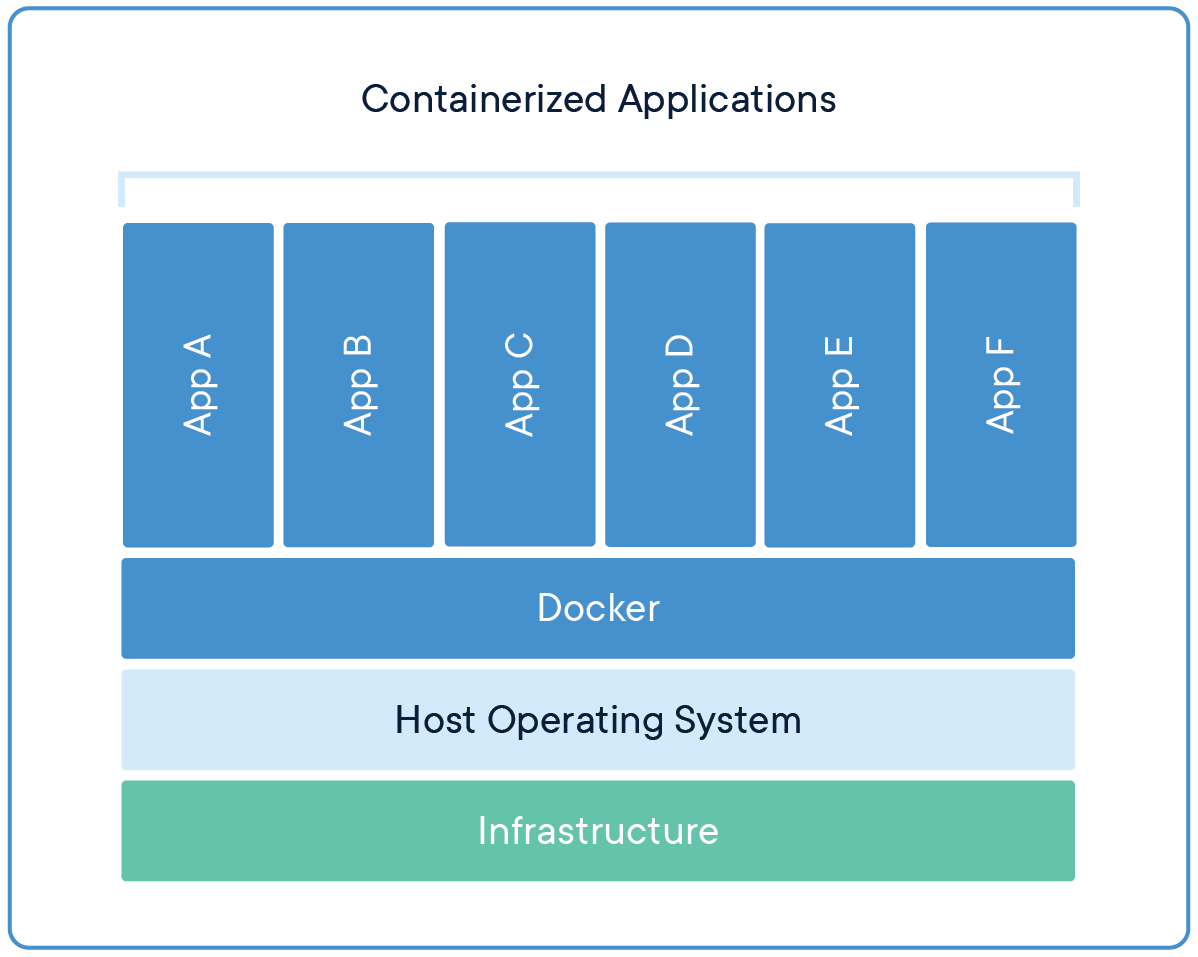
\includegraphics[width=0.6\textwidth]{docker_what_is_container.png}\\
    \cite{What_is_container}
\end{frame}

\begin{frame}
    \frametitle{Big idea}
    \centering
    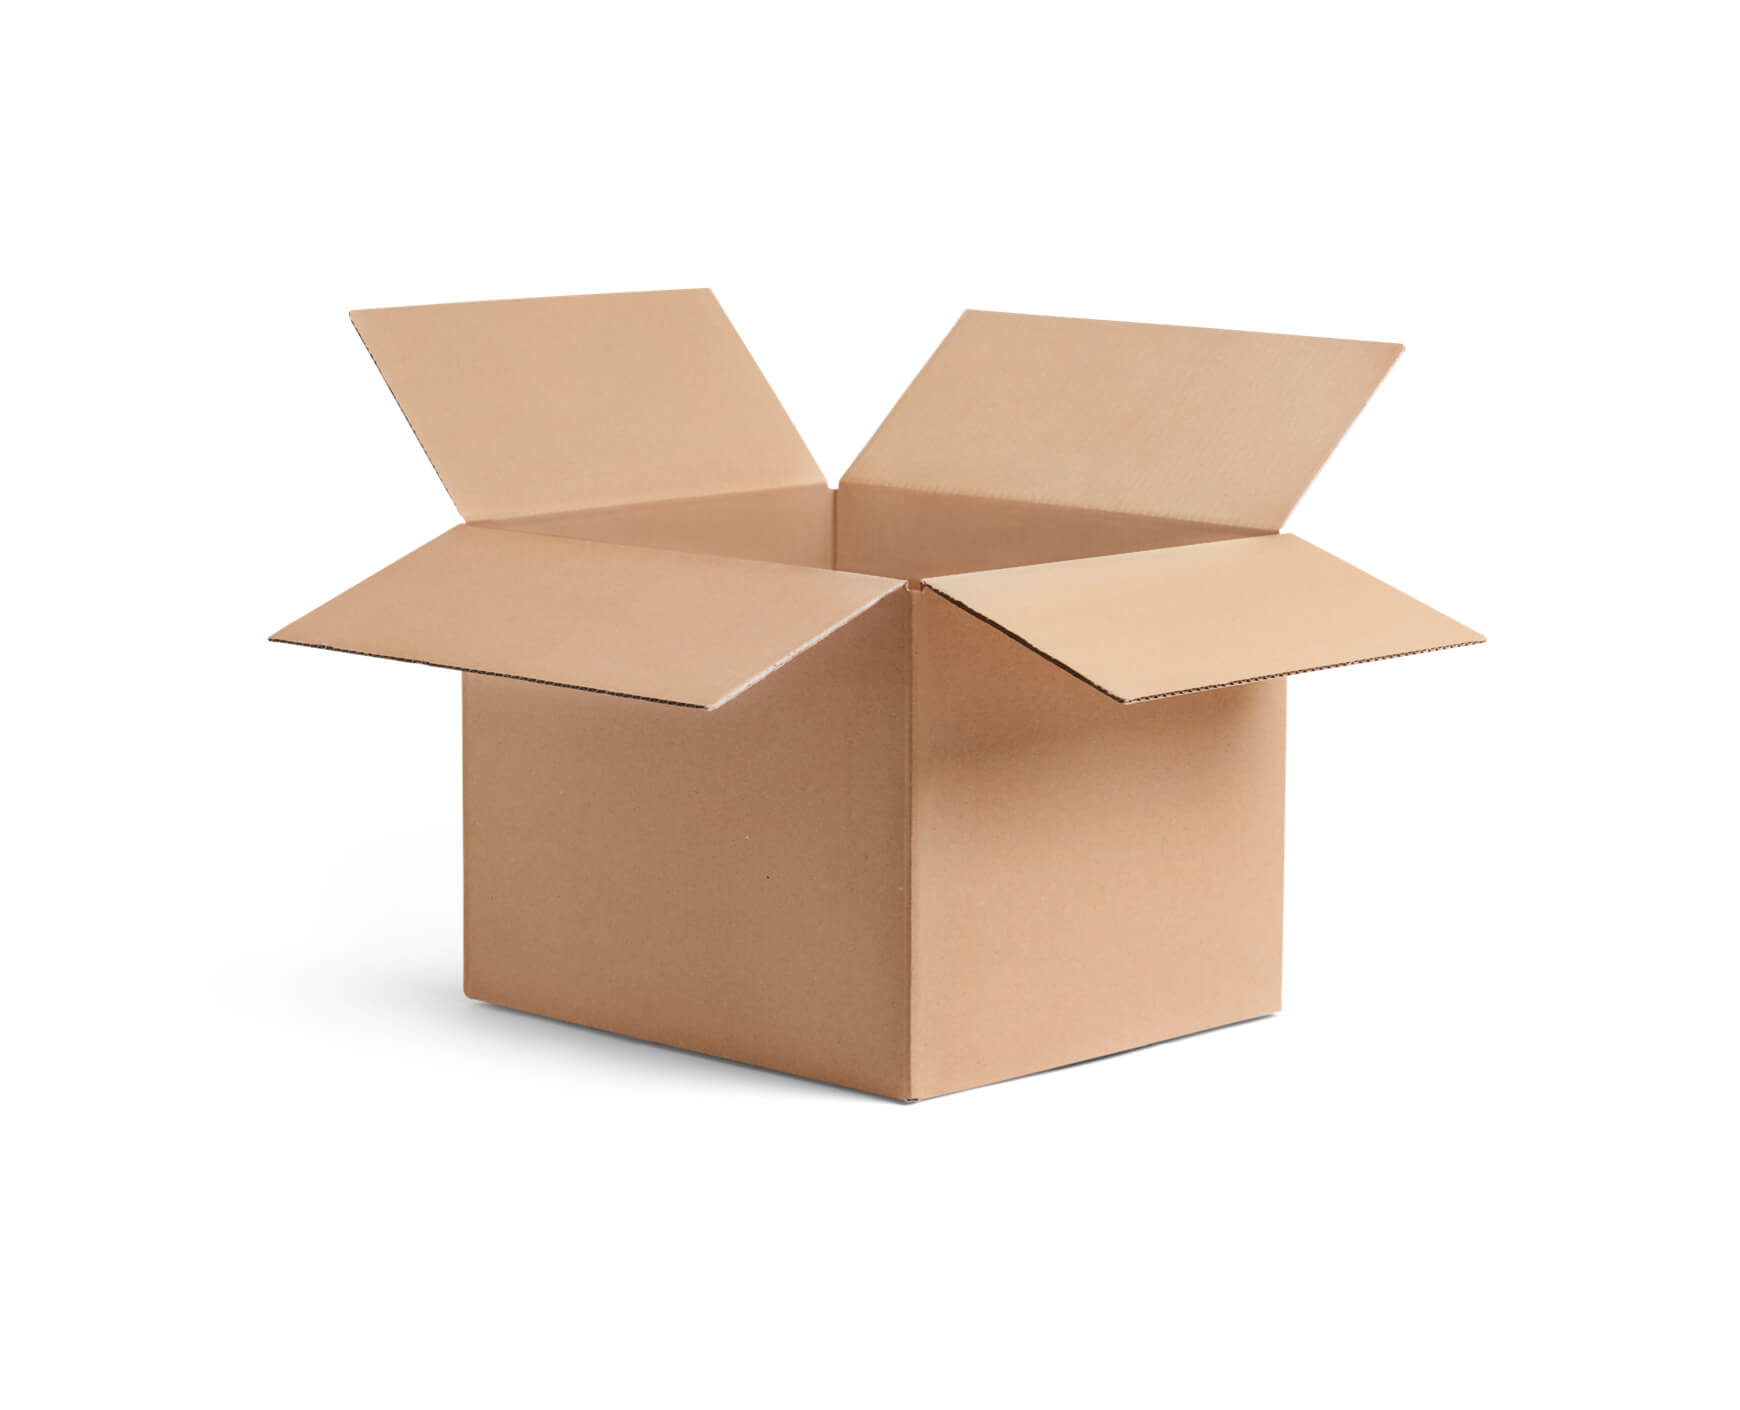
\includegraphics[width=0.8\textwidth]{box.jpg}
    \cite{box_graph}
\end{frame}

\subsection{Comparing Containers and Virtual Machines}
\begin{frame}
    \frametitle{Compare with virtule machines}
    \begin{center}
        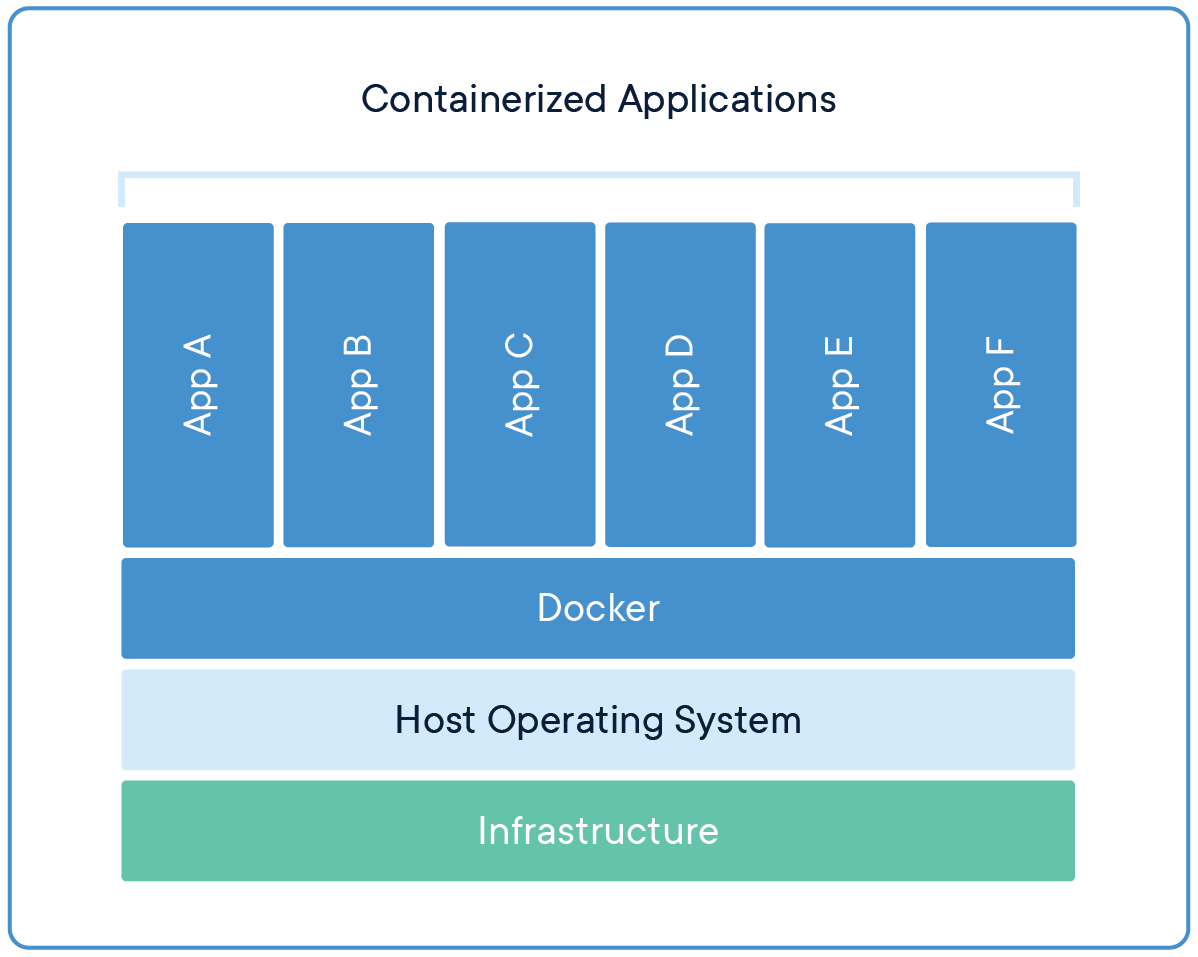
\includegraphics[width=.49\textwidth]{docker_what_is_container.png}
        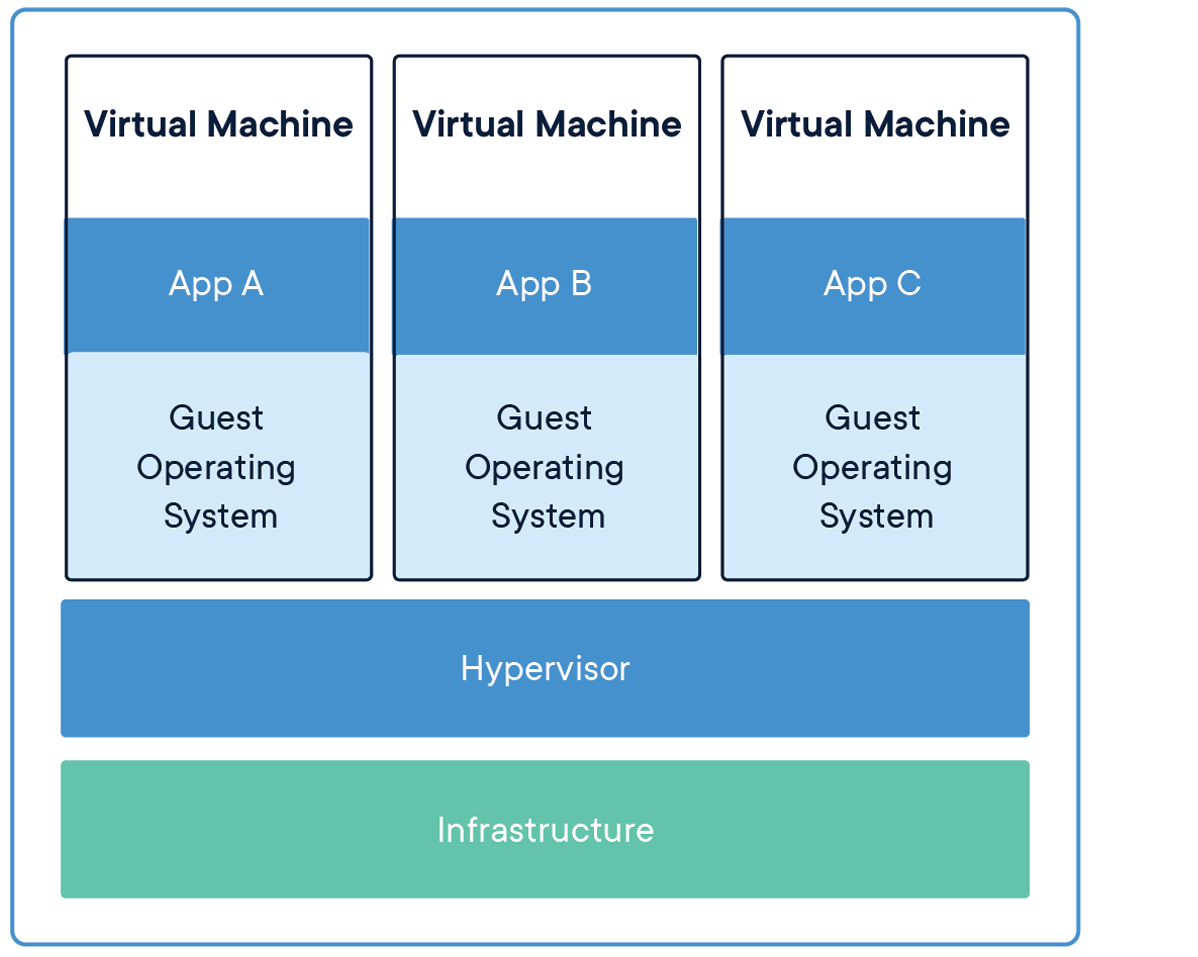
\includegraphics[width=.5\textwidth]{container-vm-whatcontainer_2.png}
    \end{center}
\end{frame}

\begin{frame}
    \frametitle{So, what is share kernel?}
    \begin{center}
        Let's recall the OS 101 course\\
        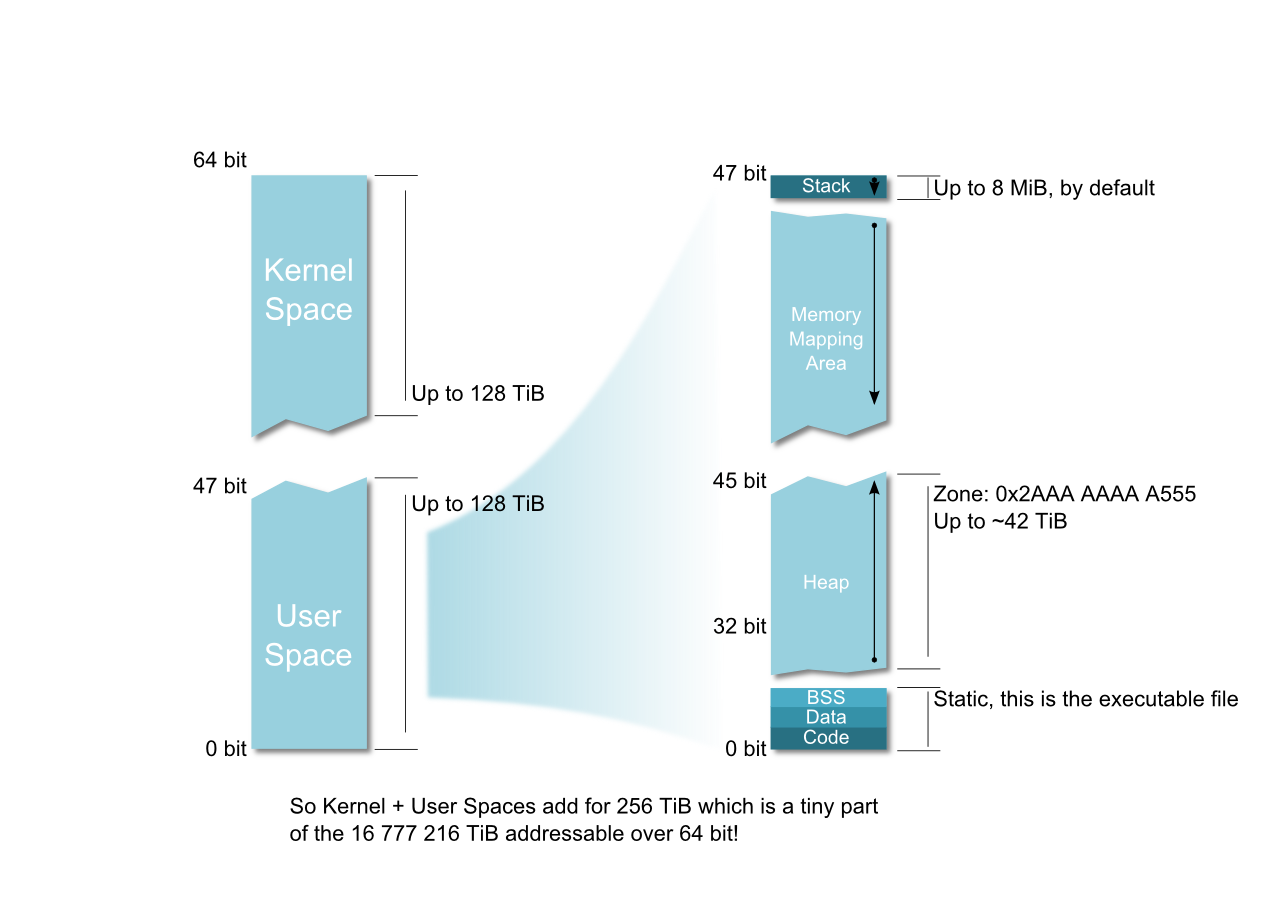
\includegraphics[width=.8\textwidth]{linux_memory_layout_64bit.png}
        \cite{64_mem_layout}
    \end{center}
\end{frame}

\begin{frame}
    \frametitle{So, what is share kernel?}
    \centering{The 32-bits memory layout}
    \begin{center}
        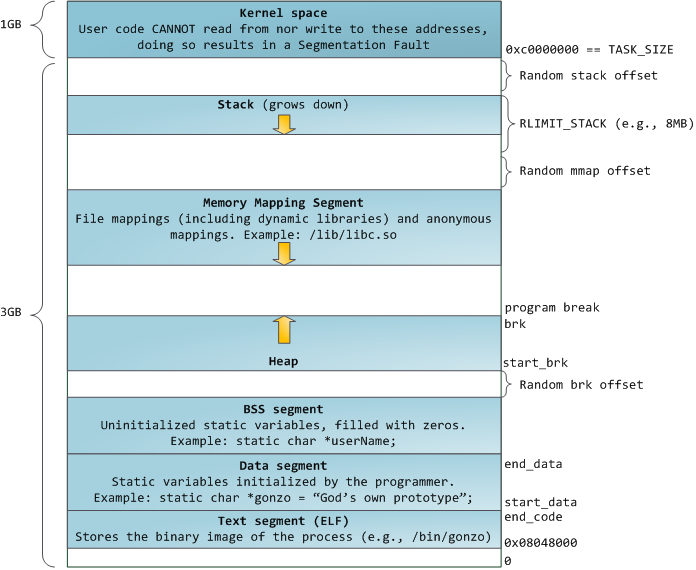
\includegraphics[width=.7\textwidth]{32bit_mem_layout.png}
        \cite{32_mem_layout}
    \end{center}
\end{frame}

\begin{frame}
    \frametitle{What is HYPERVISOR?}
    \begin{center}
        Virtual machine monitor
    \end{center}
\end{frame}

% ======================Dockerfile============================
\section{Dockerfile}
\subsection{Introduction}
\begin{frame}
    \frametitle{What is Dockerfile?}
    \begin{block}{Definition:}
        A {\color{red}{text}} document that contains all the {\color{red} commands}\
        a user could call on the command line to {\color{green} assemble an image}.
    \end{block}
\end{frame}

\begin{frame}
    \frametitle{Image and Container}
    \centering
    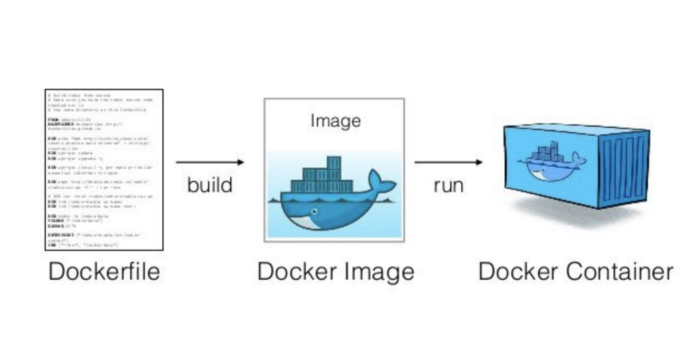
\includegraphics[width=.95\textwidth]{1_p8k1b2DZTQEW_yf0hYniXw.png}
    \cite{Build_an_image}\\
    Like a program in execution is called a process.\\
    An image in execution is called a container.
\end{frame}

\begin{frame}
    \frametitle{DockerHub}
    A public \textbf{images} hub. We push/pull \textbf{images} from it by default.\\
    We push an image and pull an image rather than a container.
    \newline
    \newline
    \begin{center}
        Make sense, right?
    \end{center}
\end{frame}

\subsection{Write a Dockerfile}
\begin{frame}
    \frametitle{Dockerfile 101}
\end{frame}

\begin{frame}
    \frametitle{Our Dockerfile}
\end{frame}

% ======================Commands============================
\section{Docker commands}
\subsection{Basic commands}
\begin{frame}
    \frametitle{Basic}
    \centering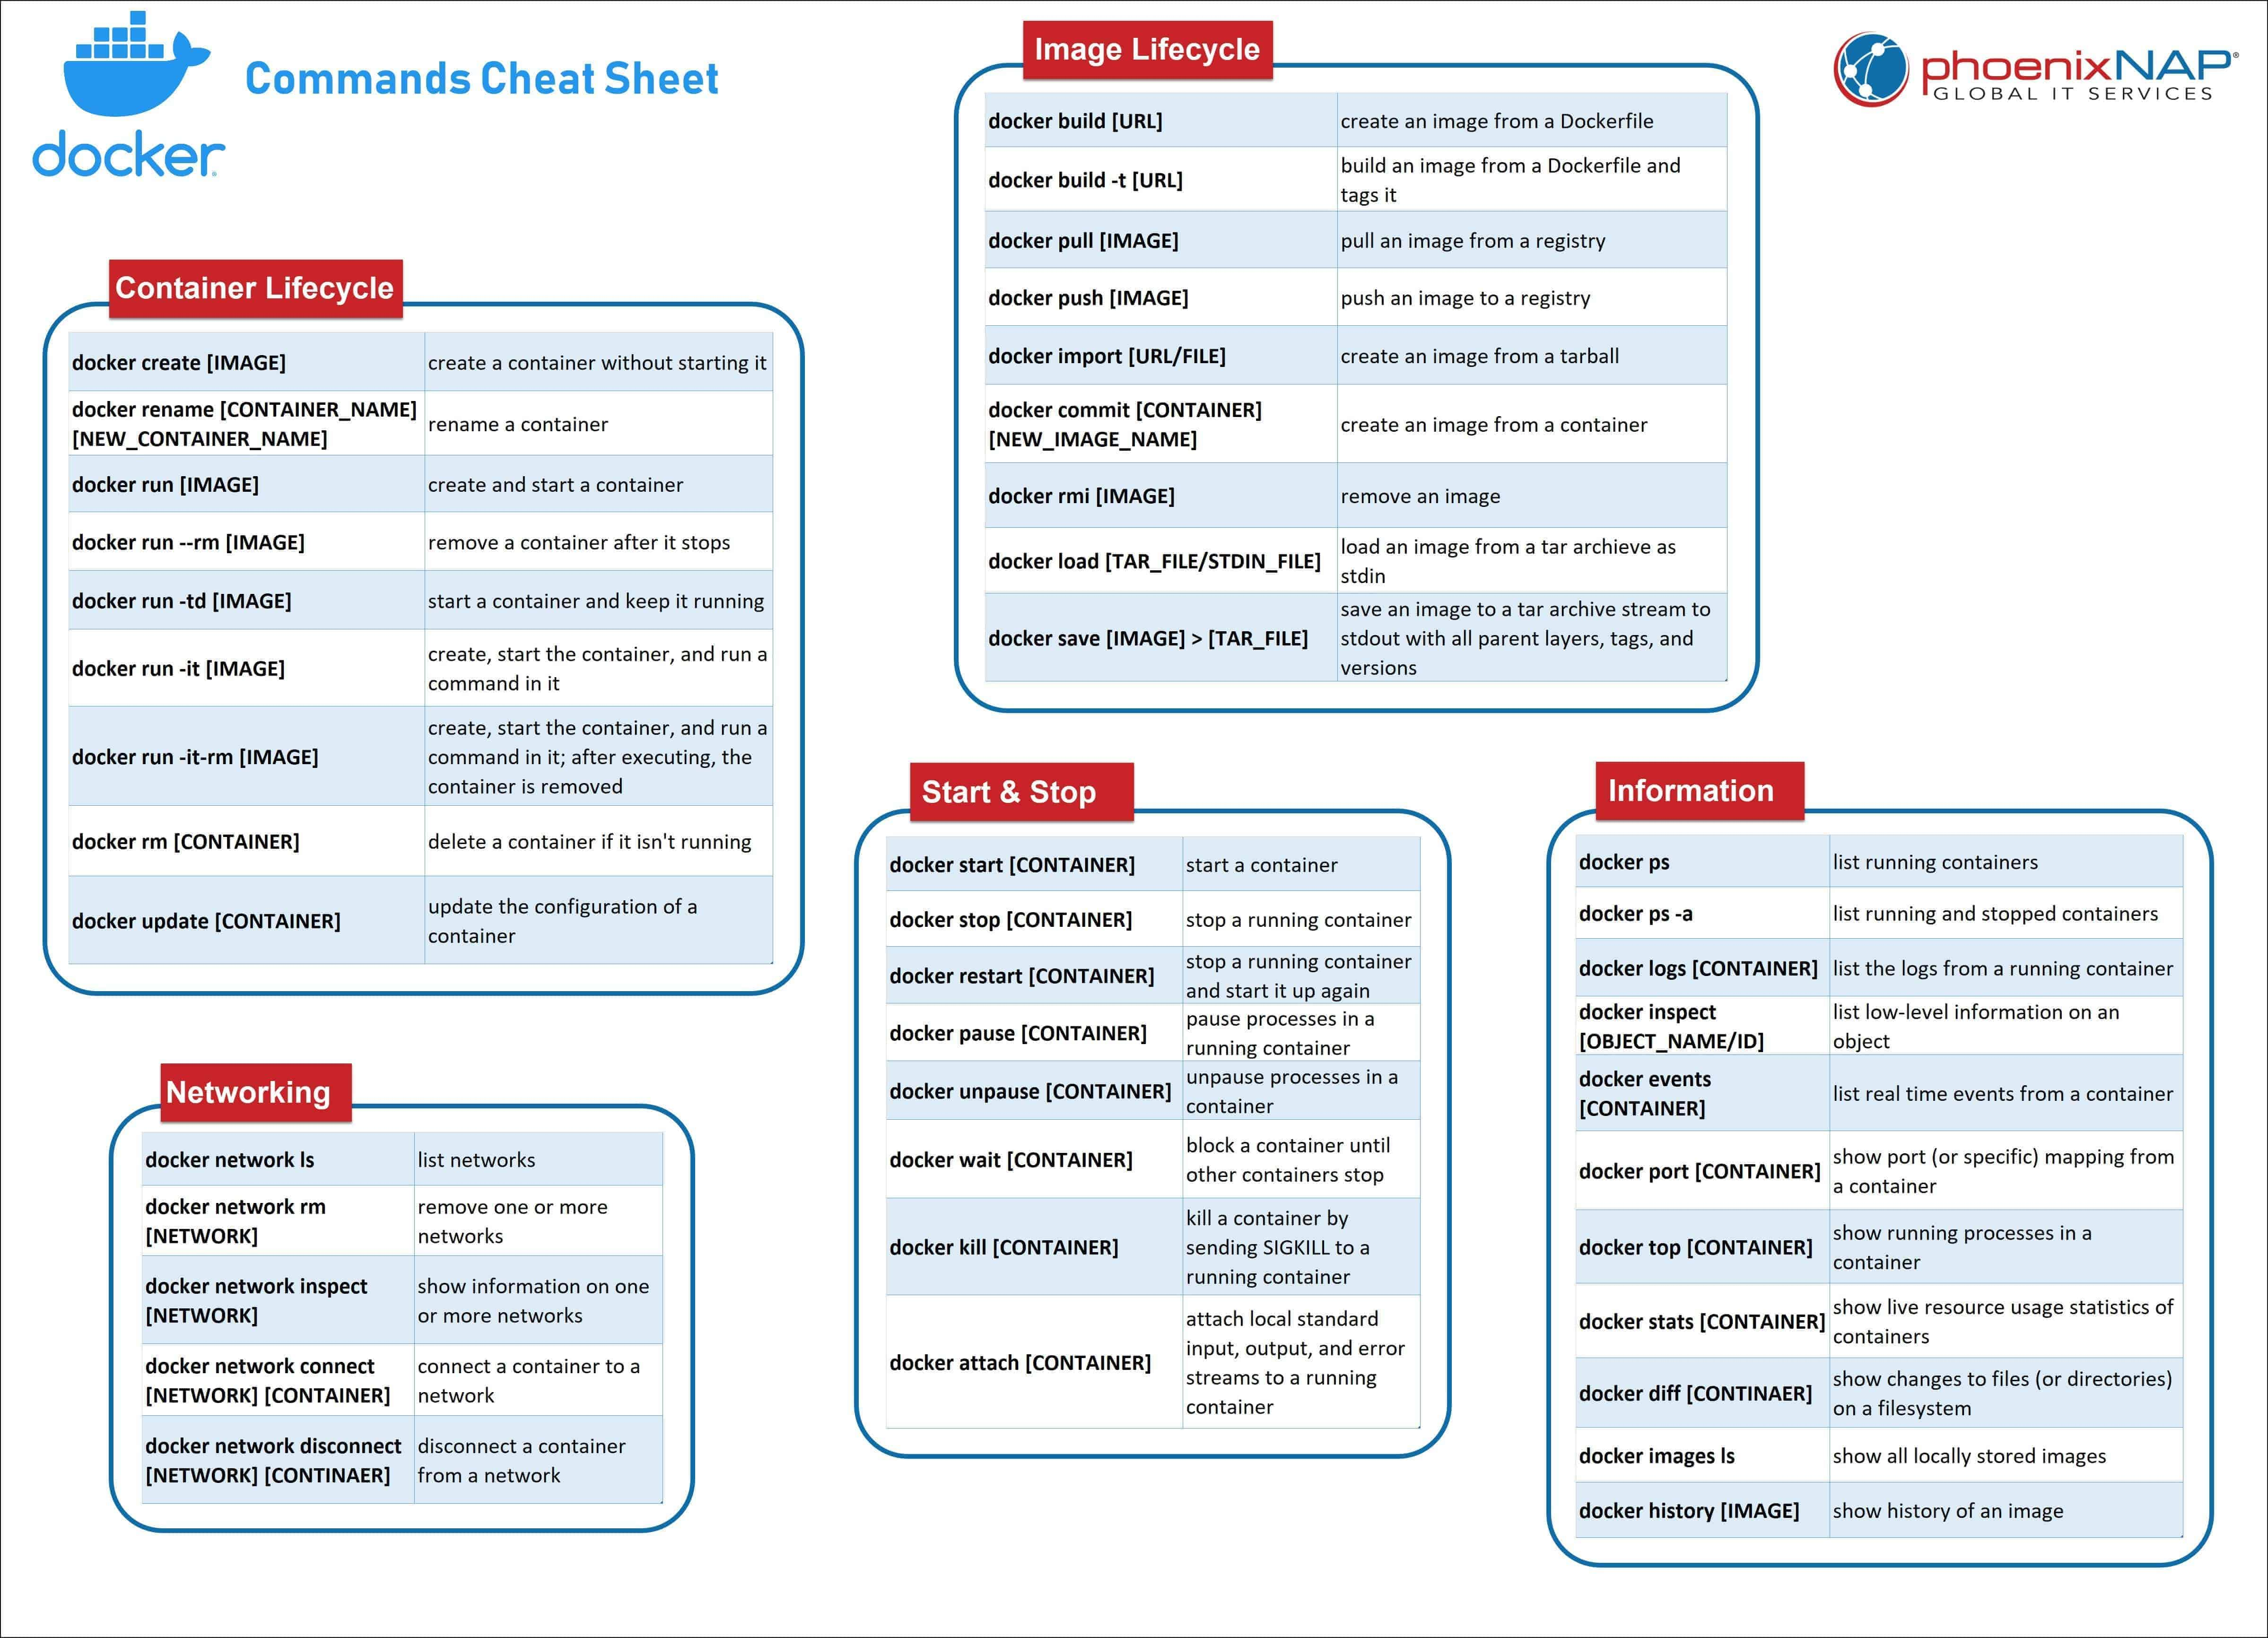
\includegraphics[height=0.9\textheight]{Docker commands cheat sheet by PhoenixNAP.jpeg}
    \cite{small_chear_sheet}
\end{frame}

\begin{frame}
    \frametitle{Full cheat sheet}
    Next page reference: \cite{cheat_sheet_full}
\end{frame}
{\setbeamercolor{background canvas}{bg=}
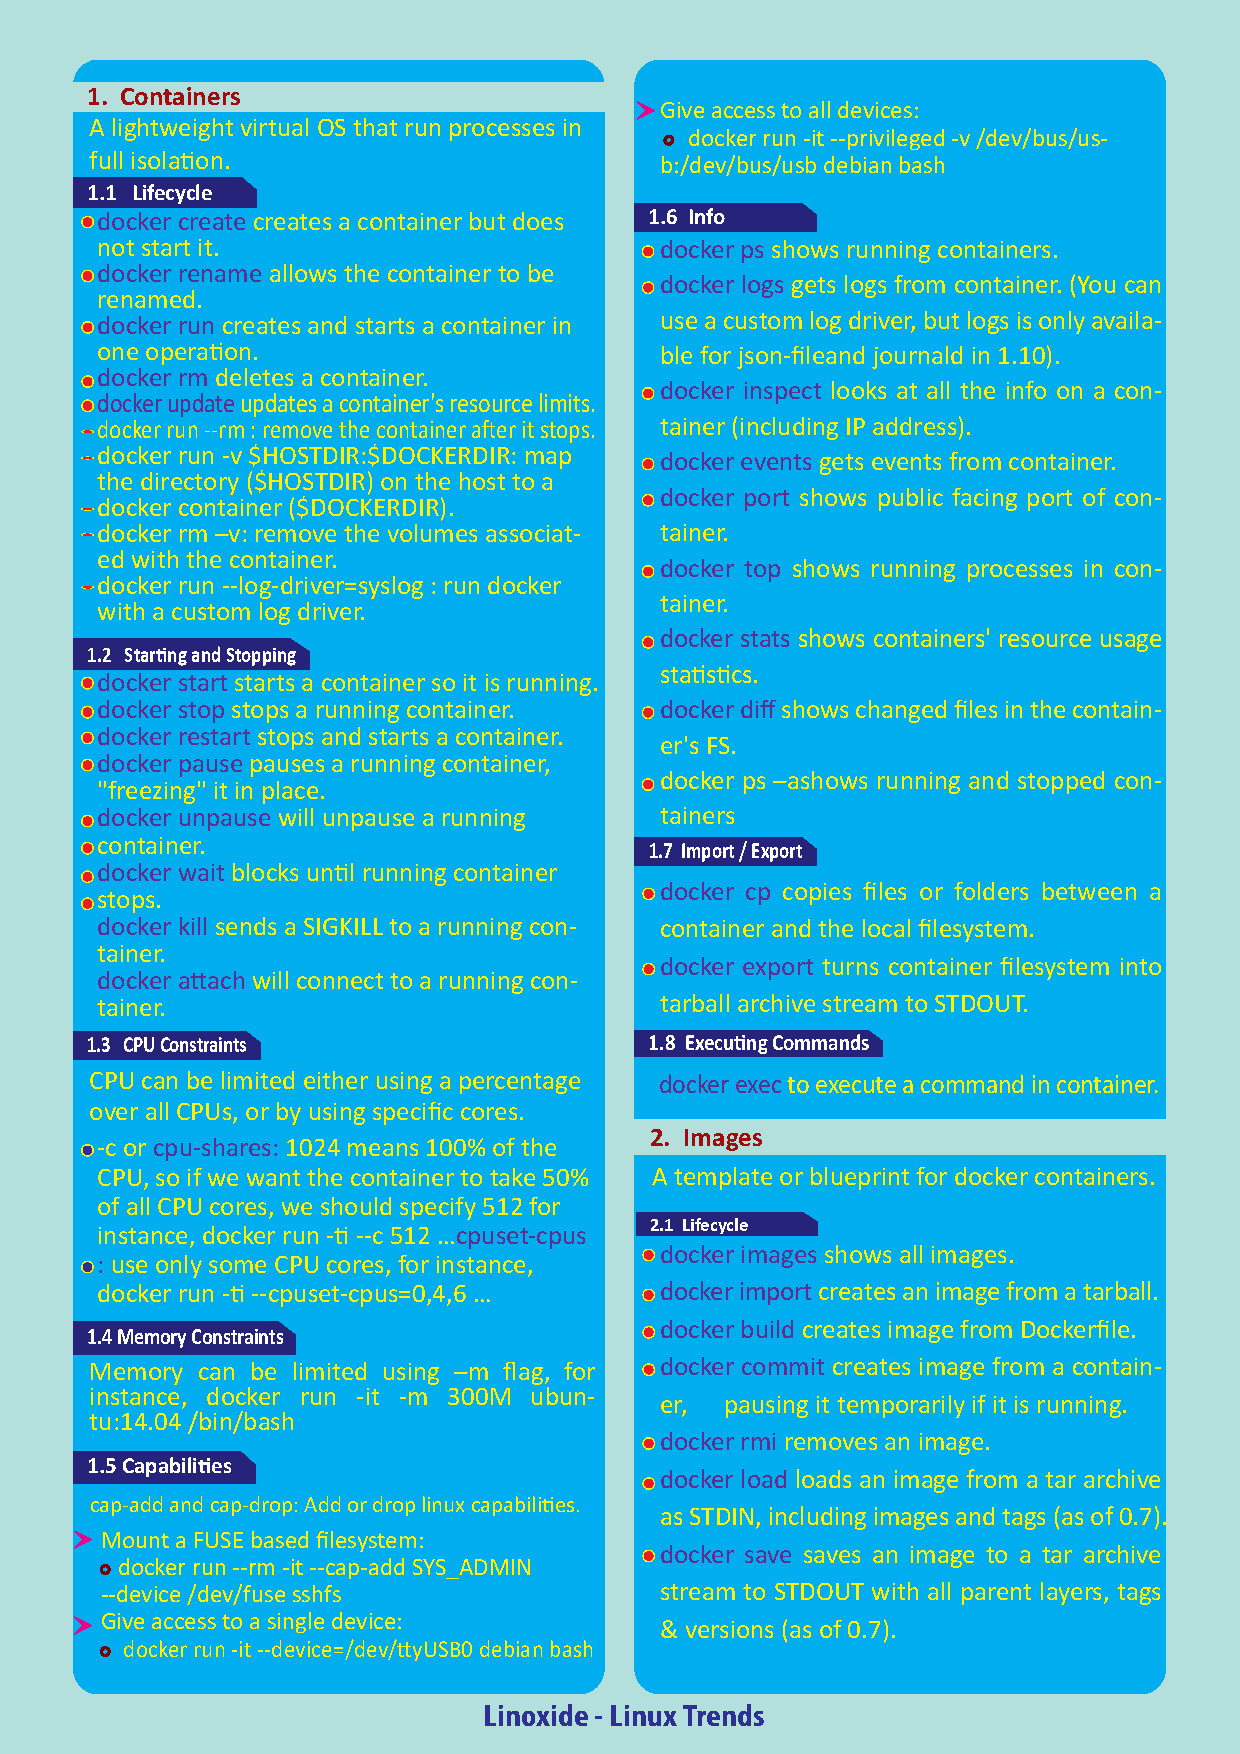
\includepdf[pages=-]{src/docker-commands-cheat-sheet.pdf}
}

\subsection{Exercises}
\begin{frame}
    \frametitle{Exercises}
\end{frame}

% ======================Goal============================
\section{Tiny project}
\begin{frame}
    \frametitle{Single-responsibility principle}
    \begin{quote}
        Why we should decompose this project into tiny-tiny parts?
    \end{quote}

    \begin{block}{Wikipedia:}
        The single-responsibility principle (SRP) is a computer-programming principle that\
        states that every class in a computer program should have responsibility over a\
        single part of that program's functionality, which it should encapsulate. All of\
        that module, class or function's services should be narrowly aligned with that\
        responsibility \cite{SRP_wiki}.
    \end{block}
\end{frame}
\subsection{Image deployment}
\begin{frame}
    \frametitle{Our Labs}
\end{frame}

\subsection{X Window forwarding}
\begin{frame}
    \frametitle{Wine with X11}
\end{frame}

\subsection{Maybe: Cross platform}
\begin{frame}
    \frametitle{Raspbian on Docker}
\end{frame}

\section{Security}

\section{References}
\begin{frame}[t, allowframebreaks]
    \frametitle{References}
    \printbibliography
\end{frame}

\end{document}